Three bright-field microscopy images datasets were acquired with the ZEISS Axiocam ERc5s camera in the ZEISS SteREO Discovery.v20 and the ZEISS AxioLab A1 stereo microscopes from the Scientific Computing Group (SCG) at São Carlos Institute of Physics (IFSC). The datasets contain images from leaf histological samples of the plants \textit{Callisia repens}, \textit{Tradescantia zebrina} and \textit{Cthenante oppenheimiana}, acquired with different focal planes and with different magnification levels. 

A shared feature between the species \textit{Callisia repens}, \textit{Tradescantia zebrina} and \textit{Cthenante oppenheimiana} is the purple abaxial (lower or bottom) leaf surface, and is commonly observed in deeply-shaded understorey plants, and might be transient or permanent depending on the species and environmental conditions \cite{filho2018plants}. Several research projects were done by the SCG group on plant leaf images, including biological studies with complex network analysis, where the locations of particular structures of the leaf, i.e. the stomata, were modeled as graphs. The \emph{stoma} (plural \emph{stomata}) is a structure that consists of an aperture between two cells, named \emph{guard cells}, and controls the exchange of steam, CO$_{2}$ and other gases from the inner part of the leaf and the atmosphere  \cite{hetherington2003role}. Furthermore, the concentration of stomata in leaves of purple plants is high; such stomatal cells are green and create a contrast between the epidermis and the stomata, which yields very good results with optical microscopy imaging \cite{filho2018plants}. Samples of blurred and sharp images of both datasets are shown in Figure \ref{fig:datasets}.

\begin{figure}[ht]
	\centering
	\caption{Examples of the proposed dataset images: blurred \textit{Callisia} \textbf{(a)}, sharp \textit{Callisia} \textbf{(b)}, blurred \textit{Tradescantia} \textbf{(c)}, sharp \textit{Tradescantia} \textbf{(d)} and blurred \textit{Cthenante} \textbf{(e)}, sharp \textit{Cthenante} \textbf{(f)}.}
	\label{fig:datasets}
	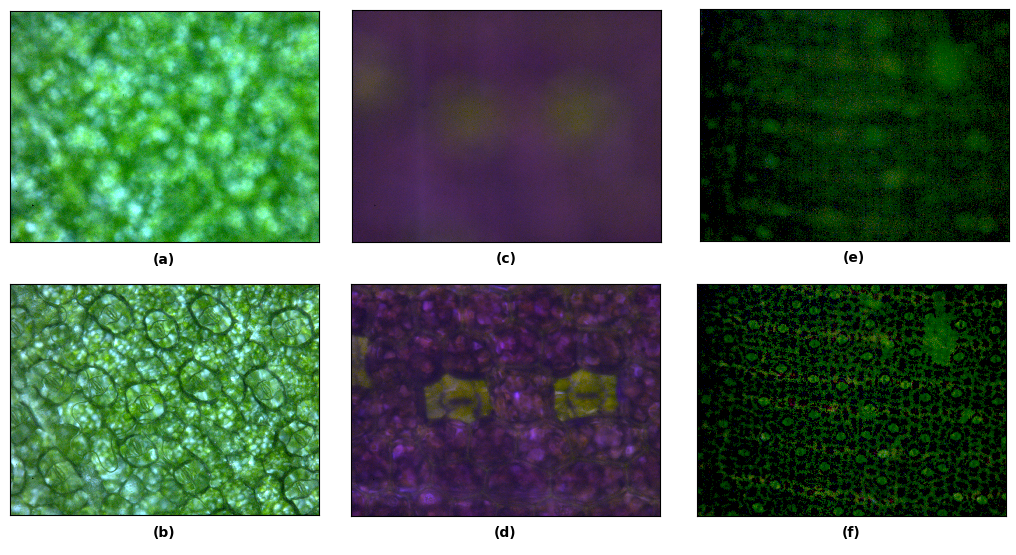
\includegraphics[scale=0.4]{images/datasets.png}
	\centering
	\fautor
\end{figure}

We will refer to the datasets as \textit{Callisia}, \textit{Tradescantia} and \textit{Cthenante} for notation simplicity. The \textit{Callisia} and \textit{Tradescantia} datasets were acquired with the z-stacking method in the SteREO Discovery.v20 microscope, endowed with a motorized drive to automatically change the focal plane by moving the objectives, whereas the \textit{Cthenante} dataset was acquired with the AxioLab A1 microscope, a standard stereo microscope which allows higher magnification levels. The workstation was connected to the microscope by means of the ZEISS Axiovision version 4.8 software package, which allows the microscope operator to manually or automatically set acquisition parameters for the z-stack acquisition, register the images, i.e. align each stack, enhance images and so on. Nevertheless, the software was a drawback for the acquisition process. The workstation went through technical problems and there was no option but to reinstall the operating system and, consequently, the Axiovision software. In order to properly configure the communication between the workstation and the microscope, an authorized technician was needed, but we did not have access to such a person. Therefore, the z-stacks were manually built.

The SteREO Discovery.v20 microscope allows a precise measurement of the objective height, and the slices were acquired with a distance of 10 $\mu$m between each other - the maximum manually achievable distance. On the other hand, the absence of such micrometer precision measurement in the AxioLab A1 microscope did not hinder the construction of the z-stacks. For both microscopes, the acquisition started with the objective height above the focal plane, which provided a completely blurred image. Then, the objective was axially lowered in steps, and for each step, an image was taken; this process was done until the objective height was below the focal plane and the images were blurred again.

The z-stacks needed to be registered for image fusion, but it only makes sense to do it after the eligible images in each set were chosen. Therefore, after our IQA method was applied, we aligned each stack with the TrakEM2 package, which is an ImageJ-based tool for processing and analyzing microscopy images, which includes methods for lens distortion correction, stitching, serial section alignment, correction of section thickness, and contrast adjustment \cite{saalfeld2019computational}. TrakEM2 uses the techniques described in the Image Registration section of Chapter~\ref{chapter:theoretical-background} to align the stacks.

In order to validate the results with correlation to a subjective quality index, each image was labeled as sharp or blurred, which respectively translates to \emph{eligible} and \emph{negligible} for the fusion process. The axial nature of the acquisition allowed for a contiguous set of eligible images in each dataset. The relevant properties of the datasets are summarized in Table \ref{tab:dataset_info}. 

\begin{table}[ht]
    \centering
    \caption{Information about the proposed datasets.}
    \label{tab:dataset_info}
    \begin{tabular}{lcccc}
        \toprule
        \textbf{Dataset} & \textbf{Images} & \textbf{Magnification} & \textbf{Sharp} & \textbf{Sequence}\\
        \midrule
        \textit{Callisia} & 56 & 50$\times$ & 9 & 41 - 49\\
        \textit{Tradescantia} & 66 & 200$\times$ & 2 & 50 - 51\\
        \textit{Cthenante} & 55 & 100$\times$ & 16 & 30 - 45\\
        \bottomrule
    \end{tabular}
    \centering
    \fautor
\end{table}